\chapter{Análisis y discusión de los resultados}
En este capítulo se exponen los resultados alcanzados en esta investigación y para ello se tomaron: un período de la cronología (1980 - 2018), algunas de las categorías del filtro (3 - 5) y una región del país (Centro), para procesar la información y observar los resultados que produce el software \textbf{TkHURSv1.1} para algunas de sus posibles salidas.\\

La primera imagen que se presenta es una parte de la cronología general (Figura \ref{fig:cronologia_general_parte}), el cambio respecto a las demás imágenes va a ser evidente porque la opción ``Cronología General'' es la única función en la aplicación de escritorio que no es afectada por los filtros

\begin{figure}[H]
\centering
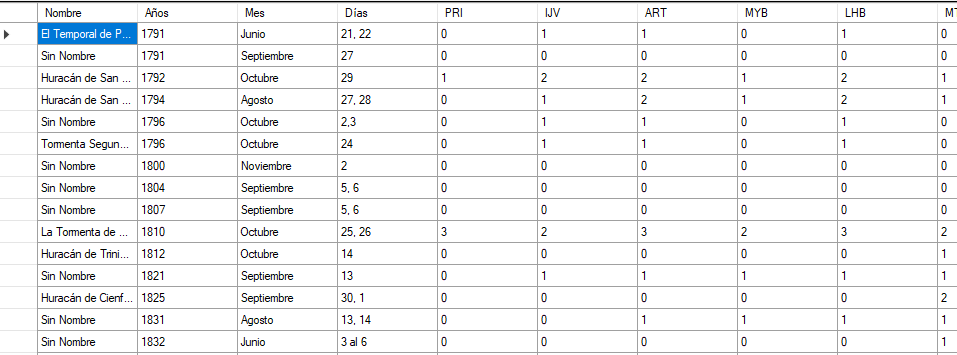
\includegraphics[scale=0.50]{cronologia_general_parte}
\caption{Fragmento de la Cronología de huracanes de Cuba (1791-2018)}
\label{fig:cronologia_general_parte}
\end{figure}

\pagebreak

La siguiente es la cronología filtrada a partir de las opciones escogidas que se mencionaron al principio (Figura \ref{fig:cronologia_filtrada19802018}). Por este resultado podemos conocer que la región Central de Cuba fue afectada por 4 huracanes en el rango de categorías elegido en la escala Saffir - Simpson durante el período de 1980 a 2018.


\begin{figure}[H]
\centering
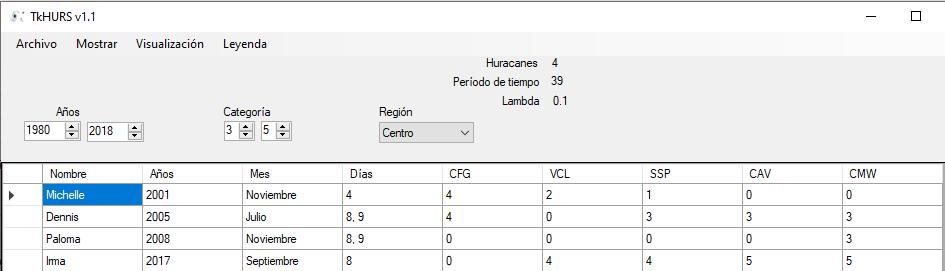
\includegraphics[scale=0.60]{cronologia_filtrada19802018}
\caption{Cronología filtrada, región Central de Cuba (1980-2018)}
\label{fig:cronologia_filtrada19802018}
\end{figure}

En la próxima imagen se muestran los huracanes por categoría (Figura \ref{fig:huracanes_categoria19802018}). Se aprecia que las categorías SS1 y SS2 tienen valor 0, resultado esperado dado que se dejaron fuera del rango de categorías seleccionado. 

\begin{figure}[H]
\centering
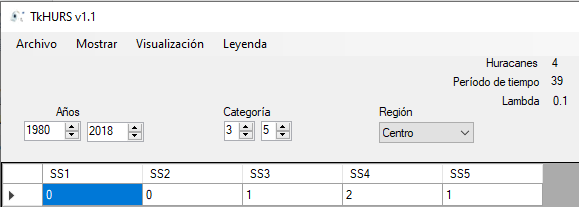
\includegraphics[scale=1]{huracanes_categoria19802018}
\caption{Huracanes por categorías intensas, región Central de Cuba (1980-2018)}
\label{fig:huracanes_categoria19802018}
\end{figure}

\pagebreak

Lo que se aprecia a continuación (Figura \ref{fig:periodos_retorno19802018}) es la tabla de períodos de retorno, donde se puede esperar que en la región Central pase un huracán intenso cada 10 años aproximadamente. %Las casillas que se exponen son las relacionadas con la prueba $\chi^{2}$ de Bondad de Ajuste, pero el usuario tiene la opción de ver los resultados relacionados con la prueba Kolmogorov-Smirnov que ya estaba disponible en el software desde la versión anterior.

\begin{figure}[H]
\centering
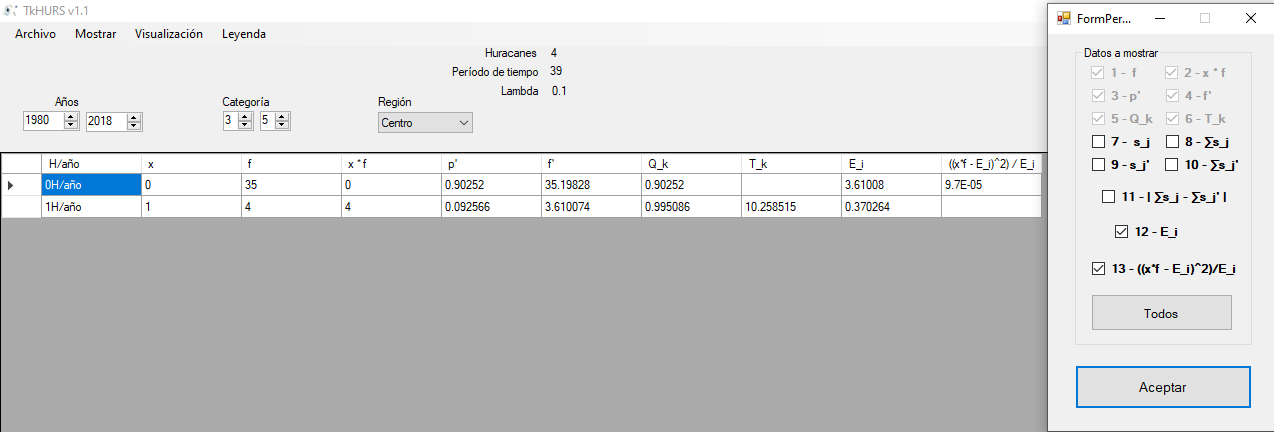
\includegraphics[scale=0.45]{periodos_retorno19802018}
\caption{Períodos de Retorno, región Central de Cuba (1980-2018)}
\label{fig:periodos_retorno19802018}
\end{figure}


El gráfico de barras muestra que en la región Central en la década del 2002-2012 fue el mas activo del período de estudio (Figura \ref{fig:barras_periodos19802018}). %Esta imagen (Figura \ref{fig:barras_periodos19802018}) muestra el gráfico de barras que se da como salida a partir de escoger dicho modo de visualización. Esto es de mucha ayuda: se observan, de manera clara, las diferencias entre los objetos de interés de estudio (intervalos de tiempo en este caso).

\begin{figure}[H]
\centering
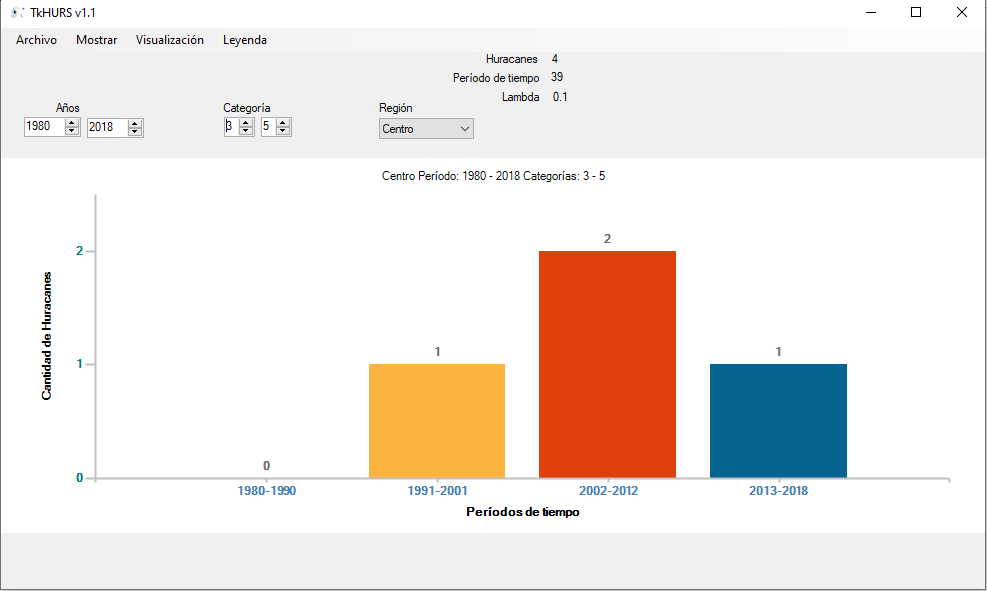
\includegraphics[scale=0.45]{barras_periodos19802018}
\caption{Gráfico de barras por décadas, región Central (1980-2018)}
\label{fig:barras_periodos19802018}
\end{figure}

\pagebreak

El gráfico de barras respecto a las provincias (Figura \ref{fig:barras_provincias19802018}) muestra como Sancti Spíritus y Camagüey han sido las más afectadas por los huracanes de categoria 3, 4 o 5 en la escala Saffir - Simpson en el período de 1980 a 2018.

\begin{figure}[H]
\centering
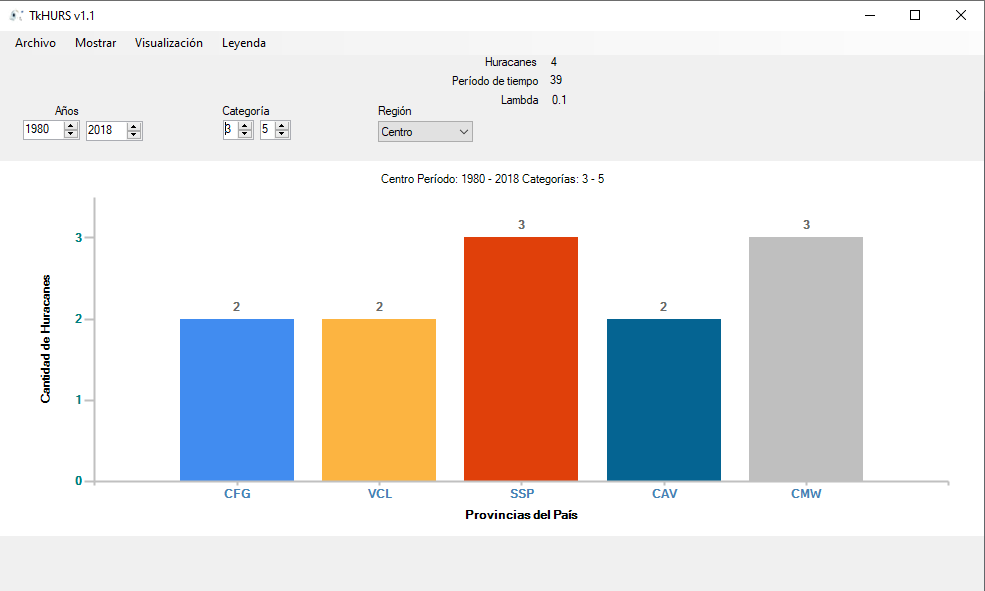
\includegraphics[scale=0.6]{barras_provincias19802018}
\caption{Gráfico de barras por provincias, región Central (1980-2018)}
\label{fig:barras_provincias19802018}
\end{figure}

\pagebreak

El gráfico de pastel en el software puede observarse en cantidad y porcentaje según se desee. Se muestra los resultados respecto a las distintas categorías: SS3, SS4 y  SS5. En este ejemplo se observa que la categoría que más ha afectado la región Central de Cuba es la cuarta (SS4) con un 50\% (Figura \ref{fig:pastel_porcentaje19802018}).%. El gráfico de pastel (Figura \ref{fig:pastel_porcentaje19802018}) solo muestra resultados respecto a las distintas categorías: SS1, SS2, SS3, SS4, SS5. Las opciones en este caso son: ``Cantidad'' y ``Porcentaje'', pero he escogido la segunda porque creo que aporta más visualmente. En este ejemplo se observa que la categoría que más ha afectado la región Central de Cuba es la cuarta (SS4) con un 50\%. 

\begin{figure}[H]
\centering
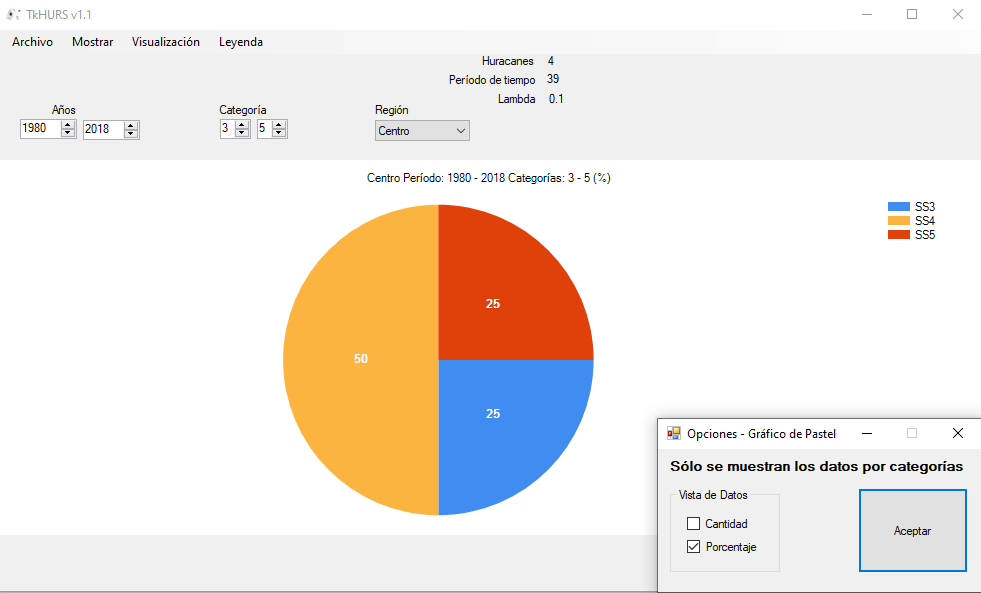
\includegraphics[scale=0.6]{pastel_porcentaje19802018}
\caption{Gráfico de pastel de las categorías en porciento, región Central (1980-2018)}
\label{fig:pastel_porcentaje19802018}
\end{figure}